%To compile as handout, use
%pdflatex "\def\ishandout{1} \input{filename.tex}"
%Defaults to non-handout mode (with slide reveals)
\ifdefined\ishandout
  \documentclass[handout]{beamer}
\else
  \documentclass{beamer}
\fi
 
\usepackage{econ103slides} 

\date{Lecture \# 2}
\begin{document} 




%%%%%%%%%%%%%%%%%%%%%%%%%%%%%%%%%%%%%%%%

\begin{frame}[plain]
	\titlepage 
	

\end{frame} 
%%%%%%%%%%%%%%%%%%%%%%%%%%%%%%%%%%%%%%%%
%\begin{frame}
%\frametitle{Some Notes on Clickers}
%
%\begin{itemize}
%	\item There was a last-minute change in the model of clicker sold at the bookstore: they now carry only the QT. Either the QT or NXT will work for this class. For more information, see
%\url{http://www.sas.upenn.edu/computing/instructional/clickers}
%	\item A clicker registration tool has been added to Canvas under ``Modules.'' Click on it and follow the instructions. 
%	\item Any votes you make before registering your clicker \emph{will still be stored}. Registering simply links your name to the unique clicker id number on the back of your remote. \alert{Just make sure to register before the drop deadline to make sure I can award you credit.}
%\end{itemize}



%\end{frame}


%%%%%%%%%%%%%%%%%%%%%%%%%%%%%%%%%%%%%%%%
\begin{frame}\frametitle{Class Survey}
 
\begin{itemize}
	\item Collect some data to analyze later in the semester.
	\item None of the questions are sensitive and your name will not be linked to your responses. I will post an anonymized version of the dataset on my website.
	\item Participation is  \emph{strictly voluntary}: you can still earn full clicker credit for today's lecture without participating in the survey.
\end{itemize}


\end{frame}


%%%%%%%%%%%%%%%%%%%%%%%%%%%%%%%%%%%%%%%%
\begin{frame}

  \frametitle{
\includegraphics[scale = 0.05]{./images/clicker}\hfill  Multiple Choice Entry -- What is your biological sex?}
\begin{enumerate}[(a)]
	\item Male
	\item Female
\end{enumerate}

\end{frame}

%%%%%%%%%%%%%%%%%%%%%%%%%%%%%%%%%%%%%%%%
\begin{frame}

\frametitle{
\includegraphics[scale = 0.05]{./images/clicker} \hfill  Numeric Entry -- How Many Credits?}

How many credits are you taking this semester? Please respond using your remote.

\end{frame}

%%%%%%%%%%%%%%%%%%%%%%%%%%%%%%%%%%%%%%%%
\begin{frame}
  \frametitle{
\includegraphics[scale = 0.05]{./images/clicker} \hfill Multiple Choice -- Class Standing} 
  What is your class standing at Penn?
  \begin{enumerate}[(a)]
    \item Freshman
    \item Sophomore
    \item Junior
    \item Senior
  \end{enumerate}
\end{frame}
%%%%%%%%%%%%%%%%%%%%%%%%%%%%%%%%%%%%%%%%
\begin{frame}
  \frametitle{
\includegraphics[scale = 0.05]{./images/clicker} \hfill Numeric Entry -- How long did you sleep?} 
  For how many hours did you sleep last night? 
  \vspace{1em}

  Please round to the nearest half hour, e.g.\ 7 hours 23 minutes becomes 7.5.
\end{frame}
%%%%%%%%%%%%%%%%%%%%%%%%%%%%%%%%%%%%%%%%

\begin{frame}
\frametitle{
\includegraphics[scale = 0.05]{./images/clicker} \hfill  Multiple Choice -- What is Your Eye Color?}
Please enter your eye color using your remote.
\begin{enumerate}[(a)]
  \item Black
  \item Blue
  \item Brown
  \item Green
  \item Gray
  \item Green
  \item Hazel
  \item Other
\end{enumerate}

\end{frame}

%%%%%%%%%%%%%%%%%%%%%%%%%%%%%%%%%%%%%%%%

\begin{frame}
\frametitle{
\includegraphics[scale = 0.05]{./images/clicker} \hfill  How Right-Handed are You?}

The sheet in front of you contains a handedness inventory. Please complete it and calculate your handedness score:
	$$\frac{\mbox{Right} -\mbox{Left}}{\mbox{Right} + \mbox{Left}}$$
When finished, enter your score using your remote.
\end{frame}

%%%%%%%%%%%%%%%%%%%%%%%%%%%%%%%%%%%%%%%%


\begin{frame}

\frametitle{
\includegraphics[scale = 0.05]{./images/clicker} \hfill  What is your Height in Inches?}

Using your remote, please enter your height in inches, rounded to the nearest inch:

\vspace{1em}
	4ft = 48in
	
	5ft = 60in 
	
	6ft = 72in
	
	7ft = 84in


\end{frame}


%%%%%%%%%%%%%%%%%%%%%%%%%%%%%%%%%%%%%%%%

\begin{frame}

\frametitle{
\includegraphics[scale = 0.05]{./images/clicker} \hfill  What is your Hand Span (in cm)?}

On the sheet in front of you is a ruler. Please use it to measure the span of your right hand in centimeters, to the nearest 1/2 cm. 

\vspace{2em}
\begin{quote}Hand Span: the distance from thumb to little finger when your fingers are spread apart\end{quote}

\vspace{2em}
When ready, enter your measurement using your remote.
\end{frame}

%%%%%%%%%%%%%%%%%%%%%%%%%%%%%%%%%%%%%%%%
\begin{frame}

\frametitle{
\includegraphics[scale = 0.05]{./images/clicker}}

We chose (by computer) a random number between 0 and 100. The number selected and assigned to you is written on the slip of paper in front of you. Please do not show your number to anyone else or look at anyone else's number.

\vspace{1em}

Please enter your number now using your remote.

\end{frame}

%%%%%%%%%%%%%%%%%%%%%%%%%%%%%%%%%%%%%%%%


\begin{frame}

\frametitle{
\includegraphics[scale = 0.05]{./images/clicker}}

Call your random number X. Do you think that the \alert{percentage} of countries, among all those in the United Nations, that are in Africa is \alert{higher} or \alert{lower} than X?

\begin{enumerate}[(a)]
	\item Higher
	\item Lower
\end{enumerate}

Please answer using your remote.

\end{frame}

%%%%%%%%%%%%%%%%%%%%%%%%%%%%%%%%%%%%%%%%

\begin{frame}
\frametitle{
\includegraphics[scale = 0.05]{./images/clicker}}
What is your best estimate of the \alert{percentage} of countries, among all those that are in the United Nations, that are in Africa?

\vspace{1em} Please enter your answer using your remote.

\end{frame}
%%%%%%%%%%%%%%%%%%%%%%%%%%%%%%%%%%%%%%%%


\begin{frame}

\Huge \centering 
Types of Variables


\end{frame}

%%%%%%%%%%%%%%%%%%%%%%%%%%%%%%%%%%%%%%%%
\begin{frame}
\frametitle{A Taxonomy of Variables}

\begin{figure}[htbp]
\begin{center}

\synttree[Variables
			[\begin{tabular}{c}Categorical\\(Qualitative)\end{tabular}
				[Nominal]
				[Ordinal]
			]%END Categorical
			[\begin{tabular}{c}Numerical\\(Quantitative)\end{tabular}
				[Interval
					[Continuous]
					[Discrete]
				]%END interval
				[Ratio
					[Continuous]
					[Discrete]
				]%END Ratio
			]%END numerical
]%END tree
%\caption{Types of Data}
%\label{fig:tree}
\end{center}
\end{figure}
\end{frame}
%%%%%%%%%%%%%%%%%%%%%%%%%%%%%%%%%%%%%%%%

\begin{frame}
\frametitle{From Weakest to Strongest}
\begin{block}{Categorical}
Qualitative, assigns each unit to category, number either meaningless or indicates order only \pause
		\begin{description}
			\item[Nominal] no order to the categories  \pause
			\item[Ordinal]  categories with natural order \pause
		\end{description}
\end{block}
\begin{block}{Numerical}
Quantitative, number meaningful \pause
		\begin{description}
			\item[Interval] only differences meaningful, no natural zero \pause
			\item[Ratio] differences and ratios meaningful, natural zero 
		\end{description}
\end{block}

\end{frame}

%%%%%%%%%%%%%%%%%%%%%%%%%%%%%%%%%%%%%%%%

\begin{frame}
\frametitle{And For Numerical Variables (interval or ratio)...}
\begin{block}{Discrete}
Takes value from discrete set of numbers, typically count data
\end{block}
\pause
\begin{block}{Continuous}
Value could be any real number within some range (even though \emph{measurements} are made with finite precision)
\end{block}

\end{frame}

%%%%%%%%%%%%%%%%%%%%%%%%%%%%%%%%%%%%%%%%
\begin{frame}
\begin{center}
\Huge
Note that in R, categorical variables are called \emph{factors}
\end{center}
\end{frame}

%%%%%%%%%%%%%%%%%%%%%%%%%%%%%%%%%%%%%%%%
\begin{frame}
\frametitle{
\includegraphics[scale = 0.05]{./images/clicker} \hfill What kind of variable is...}
...Handspan?
	\begin{enumerate}[(a)]
\item Nominal
\item Ordinal
\item Interval
\item Ratio
\end{enumerate}
\end{frame}

%%%%%%%%%%%%%%%%%%%%%%%%%%%%%%%%%%%%%%%
\begin{frame}
\frametitle{
\includegraphics[scale = 0.05]{./images/clicker} \hfill What kind of variable is...}
...Temperature?
	\begin{enumerate}[(a)]
\item Nominal
\item Ordinal
\item Interval
\item Ratio
\end{enumerate}
\end{frame}

%%%%%%%%%%%%%%%%%%%%%%%%%%%%%%%%%%%%%%%
\begin{frame}
\frametitle{
\includegraphics[scale = 0.05]{./images/clicker} \hfill What kind of variable is...}
...Eye Color?
	\begin{enumerate}[(a)]
\item Nominal
\item Ordinal
\item Interval
\item Ratio
\end{enumerate}
\end{frame}

%%%%%%%%%%%%%%%%%%%%%%%%%%%%%%%%%%%%%%%
\begin{frame}
\frametitle{
\includegraphics[scale = 0.05]{./images/clicker} \hfill What kind of variable?}
On course evaluations you can rate your professor as follows:\\ 0 = Poor, 1 = Fair, 2 = Good,  3 = Very Good, 4 = Excellent. What kind of data is your rating?
	\begin{enumerate}[(a)]
\item Nominal
\item Ordinal
\item Interval
\item Ratio
\end{enumerate}
\end{frame}
%%%%%%%%%%%%%%%%%%%%%%%%%%%%%%%%%%%%%%%
\begin{frame}
\frametitle{Handspan - Frequency and Relative Frequency}
\small
\singlespacing


\begin{columns}
    \column{0.35\textwidth}
\begin{tabular}{rrr}
cm& Freq.\ & Rel.\ Freq.\ \\
\hline
14.0         & 1 &0.01\\
17.0         & 4 &0.05\\
17.5      &  2 &0.02\\
18.0         & 5 &0.06\\
18.5      &  5 &0.06\\
19.0         & 6 &0.07\\
19.5      & 10 &0.11\\
20.0        & 10 &0.11\\
20.5      &  3 &0.03\\
21.0         & 8 &0.09\\
21.5      &  5 &0.06\\
22.0         & 9 &0.10\\
22.5      &  6 &0.07\\
23.0         & 6 &0.07\\
24.0         & 4 &0.05\\
24.5      &  3 &0.03\\
27.0         & 1 &0.01\\
\hline
& $n=89$&1.00
\end{tabular}
    \column{0.65\textwidth}
\begin{figure}
	\centering
	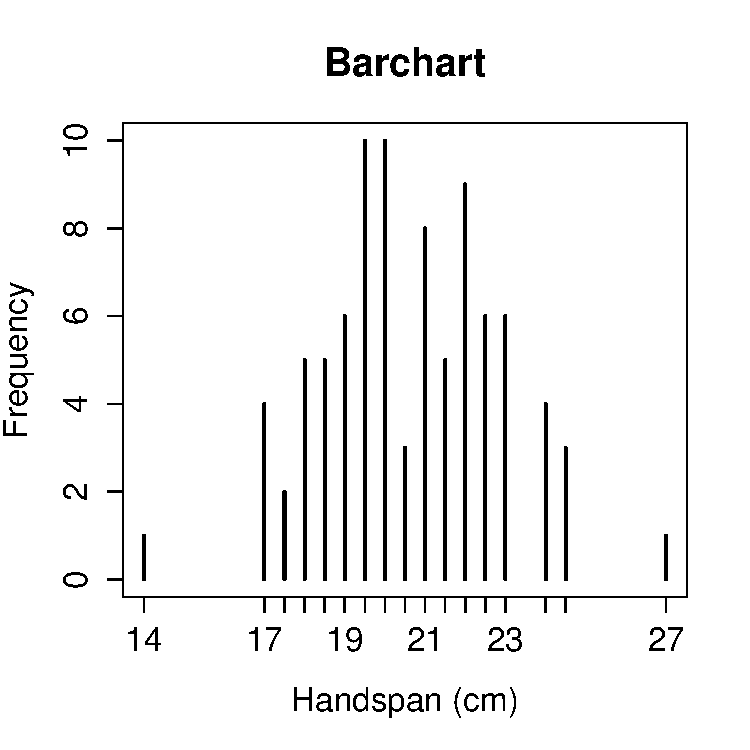
\includegraphics[scale = 0.55]{./images/handspan_freq}
\end{figure}
\end{columns}
\end{frame}
%%%%%%%%%%%%%%%%%%%%%%%%%%%%%%%%%%%%%%%
\begin{frame}
\frametitle{Handspan - Summarize Barchart by ``Smoothing''}
\small
\singlespacing


\begin{columns}
    \column{0.4\textwidth}
\begin{tabular}{rrr}
cm& Freq.\ & Rel.\ Freq.\ \\
\hline
14.0         & 1 &0.01\\
17.0         & 4 &0.05\\
17.5      &  2 &0.02\\
18.0         & 5 &0.06\\
18.5      &  5 &0.06\\
19.0         & 6 &0.07\\
19.5      & 10 &0.11\\
20.0        & 10 &0.11\\
20.5      &  3 &0.03\\
21.0         & 8 &0.09\\
21.5      &  5 &0.06\\
22.0         & 9 &0.10\\
22.5      &  6 &0.07\\
23.0         & 6 &0.07\\
24.0         & 4 &0.05\\
24.5      &  3 &0.03\\
27.0         & 1 &0.01\\
\hline
& $n=88$&1.00
\end{tabular}
    \column{0.6\textwidth}
    \alert{Group data into non-overlapping bins of equal width:}\\
    \vspace{1em}
    
\begin{tabular}{crr}
Bins & Freq.\ & Rel.\ Freq.\ \\
\hline
 $[14,16)$&1& 0.01\\
 $[16,18)$&6& 0.07\\
 $[18,20)$&26&0.30 \\
 $[20,22)$&26&0.30 \\
 $[22,24)$&21&0.24 \\
 $[24,26)$&7&0.08 \\
 $[26,28)$&1&0.01\\
 \hline
 & $n=88$&1.00
\end{tabular}
\end{columns}
\end{frame}
%%%%%%%%%%%%%%%%%%%%%%%%%%%%%%%%%%%%%%%
\begin{frame}
\frametitle{Histogram -- Density Estimate by Smoothing Barchart}
\footnotesize
\singlespacing

\begin{columns}
    \column{0.4\textwidth}
\begin{tabular}{crr}
Bins & Freq.\ & Rel.\ Freq.\ \\
\hline
 $[14,16)$&1& 0.01\\
 $[16,18)$&6& 0.07\\
 $[18,20)$&26&0.30 \\
 $[20,22)$&26&0.30 \\
 $[22,24)$&21&0.24 \\
 $[24,26)$&7&0.08 \\
 $[26,28)$&1&0.01\\
 \hline
 & $n=88$&1.00
\end{tabular}
    \column{0.6\textwidth}
\begin{figure}
	\centering
	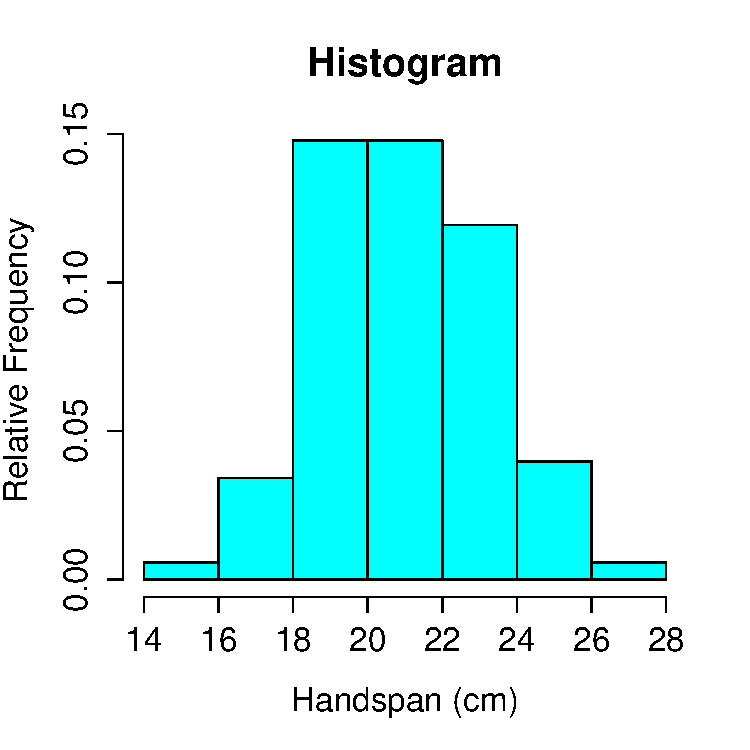
\includegraphics[scale = 0.5]{./images/handspan_truehist}
\end{figure}
\end{columns}
\end{frame}
%%%%%%%%%%%%%%%%%%%%%%%%%%%%%%%%%%%%%%%
\begin{frame}
\frametitle{Number of Bins Controls Degree of Smoothing}
\begin{figure}
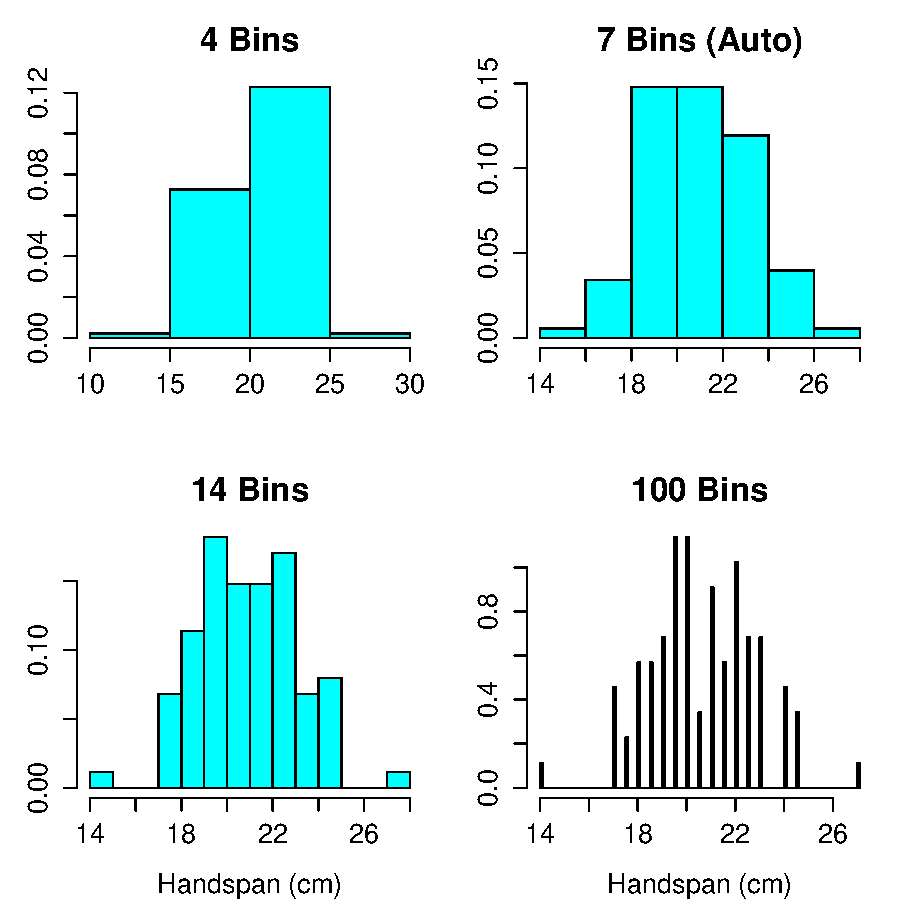
\includegraphics[scale = 0.53]{./images/handspan_four_histograms}
\end{figure}
\end{frame}
%%%%%%%%%%%%%%%%%%%%%%%%%%%%%%%%%%%%%%%
\begin{frame}
\frametitle{Histograms are \emph{Really} Important}

\begin{block}{Why Histogram?}
Summarize numerical data, especially continuous (few repeats)
\end{block}
\pause
\begin{block}{Too Many Bins -- Undersmoothing}
No longer a summary (lose the shape of distribution)
\end{block}
\pause
\begin{block}{Too Few Bins -- Oversmoothing}
Miss important detail
\end{block}
\pause
\begin{alertblock}{Don't confuse with barchart!}
\end{alertblock}
\end{frame}


%%%%%%%%%%%%%%%%%%%%%%%%%%%%%%%%%%%%%%%

\begin{frame}
\frametitle{Summary Statistic: Numerical Summary of Sample}
	\begin{enumerate}
\item Measures of Central Tendency
	\begin{itemize}
\item Mean
\item Median
\end{itemize}\pause
\item Measures of Spread
	\begin{itemize}
\item Variance
\item Standard Deviation
\item Range
\item Interquartile Range (IQR)
\end{itemize} \pause
\item Measures of Symmetry
	\begin{itemize}
		\item Skewness
	\end{itemize} \pause
\item Measures of relationship between variables 
	\begin{itemize}
\item Covariance
\item Correlation
\item Regression
\end{itemize}
\end{enumerate}
\end{frame}
%%%%%%%%%%%%%%%%%%%%%%%%%%%%%%%%%%%%%%%
\begin{frame}
\frametitle{Questions to Ask Yourself about Each Summary Statistic}
\begin{enumerate}
\item What does it measure?
\item What are its units compared to those of the data?
\item (How) do its units change if those of the data change?
\item What are the benefits and drawbacks of this statistic?
\end{enumerate}

\vspace{2em}
\alert{Some of the information regarding items 2 and 3 is on the homework rather than in the slides because working it out for yourself is a good way to check your understanding.}
\end{frame}
%%%%%%%%%%%%%%%%%%%%%%%%%%%%%%%%%%%%%%%
\begin{frame}
\frametitle{Measures of Central Tendency}
Suppose we have a dataset with observations $x_1, x_2, \hdots, x_n$
	\begin{block}{Sample Mean}
		\begin{itemize}
			\item $\displaystyle\bar{x} = \frac{1}{n} \sum_{i=1}^n x_i$
			\item Only for numeric data
			\item Works best when data are symmetric and there are no outliers
		\end{itemize}
	\end{block}\pause
	\begin{block}{Sample Median}
		\begin{itemize}
		\item Middle observation if $n$ is odd, otherwise the mean of the two observations closest to the middle.
		\item Applicable to numerical or ordinal data
		\item Robust to outliers and skewness
		\end{itemize}
	\end{block}
\end{frame}
%%%%%%%%%%%%%%%%%%%%%%%%%%%%%%%%%%%%%%%
\begin{frame}
\frametitle{Percentage of UN Countries that are in Africa}
\begin{block}{You Were a Subject in a Randomized Experiment!}
	\begin{itemize}
		\item There were only two numbers in the bag: 10 and 65
		\item Randomly assigned to Low group (10) or High group (65)
	\end{itemize}
	\end{block} \pause
\begin{block}{Anchoring Heuristic \href{http://www.jstor.org/stable/1738360}{\fbox{(Kahneman and Tversky, 1974)}}}
	Subjects' estimates of an unknown quantity are influenced by an irrelevant previously supplied starting point.
\end{block}
\begin{alertblock}{Are Penn students subject to to this cognitive bias?}
\end{alertblock}
\end{frame}
%%%%%%%%%%%%%%%%%%%%%%%%%%%%%%%%%%%%%%%
\begin{frame}
\begin{block}{Last Semester's Class}
	\begin{table}[h]
		\begin{tabular}{r|cc}
					& Mean & Median\\
					\hline
			Low ($n=43$)& 17.1&17\\
			High ($n=46$)& 30.7&30
		\end{tabular}
	\end{table}
\end{block}
\pause
\begin{block}{\href{http://www.jstor.org/stable/1738360}{\fbox{Kahneman and Tversky (1974)}}}
Low Group (shown 10) $\rightarrow$ median answer of 25\\
High Group (shown 65) $\rightarrow$ median answer of 45
\end{block}

\vspace{2em}
\alert{ \footnotesize (Kahneman shared 2002 Economics Nobel Prize with Vernon Smith.)}
\end{frame}
%%%%%%%%%%%%%%%%%%%%%%%%%%%%%%%%%%%%%%%

\begin{frame}
\frametitle{What is an Outlier?}
	\begin{block}{Outlier}
	A very unusual observation relative to the other observations in the dataset (i.e.\ very small or very big).
\end{block}
\end{frame}


%%%%%%%%%%%%%%%%%%%%%%%%%%%%%%%%%%%%%%%%
\begin{frame}
\frametitle{Mean is Sensitive to Outliers, Median Isn't}

\begin{block}{First Dataset: $\begin{array}{ccccc}1& 2& 3& 4& 5\end{array}$}
Mean = 3, Median = 3
\end{block}
\pause

\begin{block}{Second Dataset: $\begin{array}{ccccc}1& 2& 3& 4& 4990\end{array}$}
Mean = 1000, Median = 3
\end{block}
\pause
\begin{alertblock}{When Does the Median Change?}Ranks would have to change so that 3 is no longer in the middle.\end{alertblock}

\end{frame}
%%%%%%%%%%%%%%%%%%%%%%%%%%%%%%%%%%%%%%%%
\begin{frame}
\frametitle{Percentiles (aka Quantiles) -- Generalization of Median}
\begin{center}\fbox{Approx.\ $P\%$ of the data are at or below the $P^{th}$ percentile.} \end{center}
\vspace{1.5em}
\begin{block}{Percentiles (aka Quantiles)}
$P^{th}$ Percentile = Value in  $\left(P/100\right)\cdot (n+1)^{th}$ Ordered Position
\end{block}
\pause
\begin{block}{Quartiles}
Q1 = 25th Percentile

Q2 =  Median (i.e.\ 50th Percentile)

Q3 = 75th Percentile
\end{block}

\end{frame}

%%%%%%%%%%%%%%%%%%%%%%%%%%%%%%%%%%%%%%%%

\begin{frame}
\frametitle{An Example: n = 12}
$$\begin{array}{cccccccccccc}
60&63&\alert{65}&\alert{67}&70&72&75&75&80&82&84&85
\end{array}$$

\begin{eqnarray*}\mbox{Q}_1 &=& \mbox{value in the } 0.25(n+1)^{th}\mbox{ ordered position}\\\pause
	&=& \mbox{value in the } 3.25^{th}\mbox{ ordered position}\\\pause
	&=& 65 + 0.25 * (67 - 65)\\\pause
	&=& 65.5
\end{eqnarray*}
\end{frame}

%%%%%%%%%%%%%%%%%%%%%%%%%%%%%%%%%%%%%%%%

\begin{frame}
\frametitle{
\includegraphics[scale = 0.05]{./images/clicker} \hfill  Student Debt}
Guess the \alert{90th percentile} of student loan debt in the U.S. That is, guess the amount of money such that 10\% college students graduate with \emph{more} than this amount of debt and 90\% graduate with less than or equal to this amount of debt.

\end{frame}
%%%%%%%%%%%%%%%%%%%%%%%%%%%%%%%%%%%%%%%%
\begin{frame}
\frametitle{
\includegraphics[scale = 0.05]{./images/clicker} \hfill  Student Debt}

Would you guess that the median amount of student loan debt in the U.S.\ is above, below,  or equal to the mean amount?
\begin{enumerate}[(a)]
	\item Median $>$ Mean
	\item Median $=$ Mean
	\item Median $<$ Mean
\end{enumerate}

\end{frame}
%%%%%%%%%%%%%%%%%%%%%%%%%%%%%%%%%%%%%%%%
\begin{frame}
\frametitle{\footnotesize Source: \href{http://www.aeaweb.org/articles.php?doi=10.1257/jep.26.1.165}{\fbox{Avery \& Turner (2012)}}}


\centering 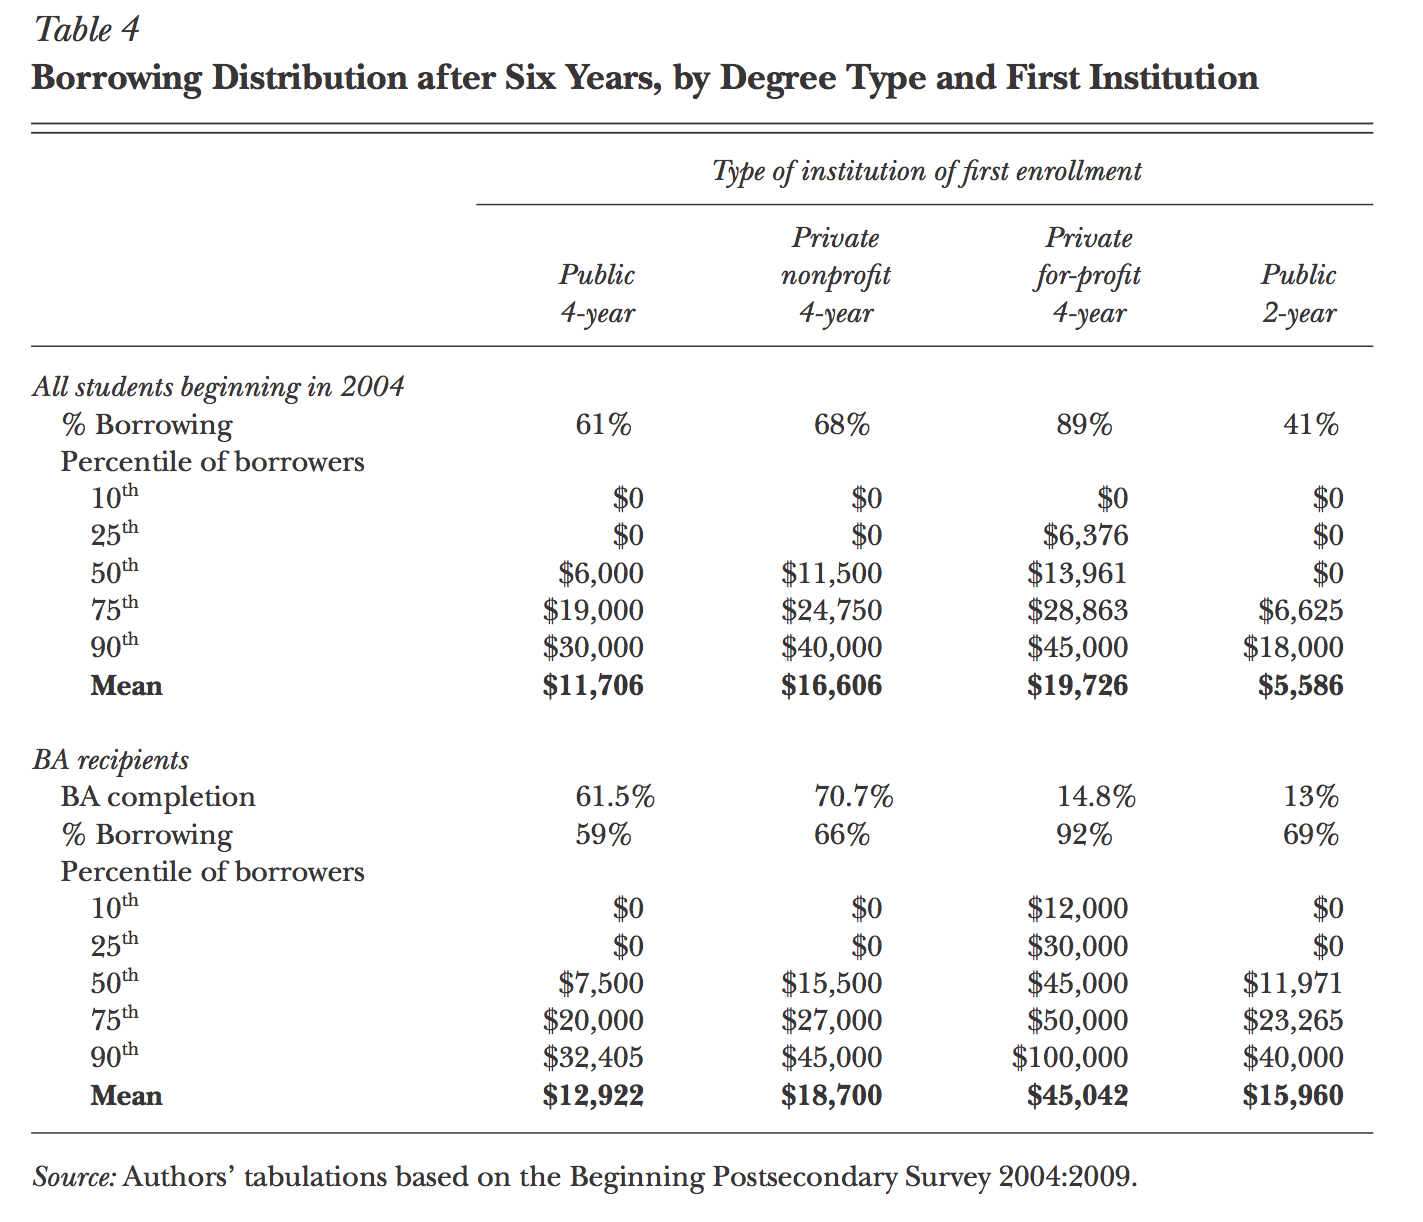
\includegraphics[scale = 0.18]{./images/student_borrowing}


\end{frame}


%%%%%%%%%%%%%%%%%%%%%%%%%%%%%%%%%%%%%%%%

\begin{frame}
\frametitle{Boxplots and the Five-Number Summary}
Minimum $<$ Q1 $<$ Median $<$ Q3 $<$ Maximum

\begin{figure}
\centering 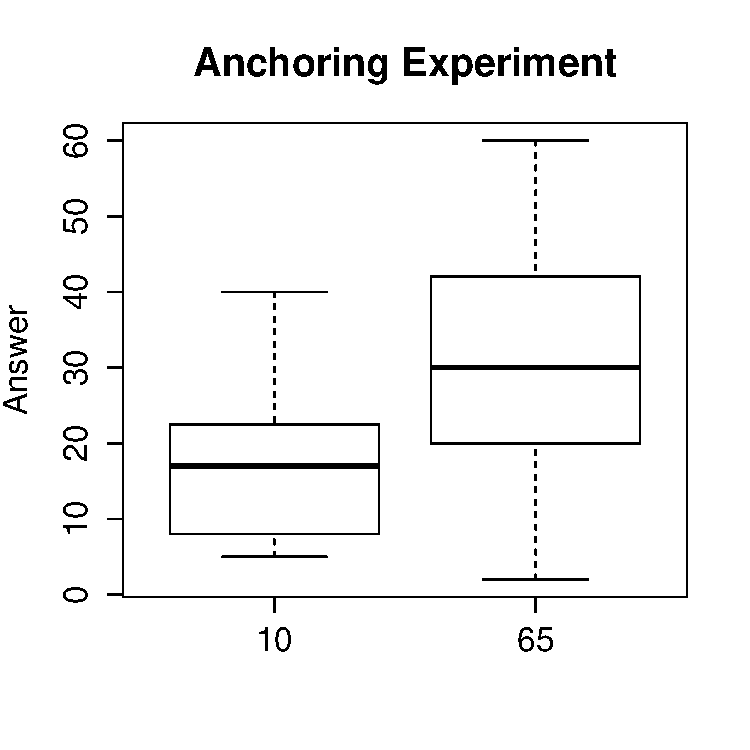
\includegraphics[scale = 0.65]{./images/anchoring_boxplot}
\end{figure}

\end{frame}
%%%%%%%%%%%%%%%%%%%%%%%%%%%%%%%%%%%%%%%%

\begin{frame}
\frametitle{Measures of Variability/Spread}

\begin{block}{Range}
Maximum Observation - Minimum Observation
\end{block}
\pause
\begin{block}{Interquartile Range (IQR)}
IQR= $\mbox{Q}_3 - \mbox{Q}_1$
\end{block}
\pause
\begin{block}{Variance}
$\displaystyle s^2 = \frac{1}{n-1} \sum_{i=1}^n (x_i - \bar{x})^2$
\end{block}
\pause
 \begin{block}{Standard Deviation}
	$s = \sqrt{s^2}$
\end{block}
\end{frame}
%%%%%%%%%%%%%%%%%%%%%%%%%%%%%%%%%%%%%%%%

\begin{frame}
\begin{block}{Variance}
Essentially the average squared distance from the mean. Sensitive to both skewness and outliers.
\end{block}
\pause
\begin{block}{Standard Deviation}
$\sqrt{\mbox{Variance}}$, but more convenient since \alert{same units as data}
\end{block}
\pause
\begin{block}{Range}
Difference between larges and smallest observations. \emph{Very} sensitive to outliers. Displayed in boxplot.
\end{block}
\pause
\begin{block}{Interquartile Range}
Range of middle 50\% of the data. Insensitive to outliers, skewness. Displayed in boxplot.
\end{block}

\end{frame}

% %%%%%%%%%%%%%%%%%%%%%%%%%%%%%%%%%%%%%%%%

% \begin{frame}
% \frametitle{Measures of Spread for Anchoring Experiment}
% \framesubtitle{Last Semester's Data}

% \begin{table}
% 	\begin{tabular}{l|cc}
% 	Treatment: & X = 10 & X = 65\\
% 	\hline
% 		Range&35&58\\
% 		IQR&14.5&21\\
% 		S.D.&9.3&15.9\\
% 		Var.&86.1&253.5
% 	\end{tabular}
% \end{table}
% \end{frame}


% %%%%%%%%%%%%%%%%%%%%%%%%%%%%%%%%%%%%%%%%
% \begin{frame}
% \frametitle{Why Squares?}
% \begin{center}\fbox{$\displaystyle s^2 = \frac{1}{n-1}\sum_{i=1}^n(x_i - \bar{x})^2$}\end{center}
% \begin{alertblock}{What's Wrong With This?}
% 	\begin{eqnarray*}
% 		\displaystyle\frac{1}{n-1}\sum_{i=1}^N (x_i - \bar{x}) &=& \pause\frac{1}{n-1}\left[\sum_{i=1}^n x_i - \sum_{i=1}^n \bar{x} \right] = \pause\frac{1}{n-1}\left[ \sum_{i=1}^n x_i  - n\bar{x}\right]\\
% 			&=& \pause \frac{1}{n-1}\left[ \sum_{i=1}^n x_i  - n\cdot\frac{1}{n} \sum_{i=1}^n x_i\right]\\ &=& \pause \frac{1}{n-1}\left[ \sum_{i=1}^n x_i  -  \sum_{i=1}^n x_i\right] =\pause 0
% 	\end{eqnarray*}
% \end{alertblock}

% \end{frame}
% %%%%%%%%%%%%%%%%%%%%%%%%%%%%%%%%%%%%%%%%

% \begin{frame}
% \frametitle{Variance is Sensitive to Skewness and Outliers}
% \framesubtitle{And so is Standard Deviation!}
% \begin{center}\fbox{$\displaystyle s^2 = \frac{1}{n-1}\sum_{i=1}^n(x_i - \bar{x})^2$}\end{center}


% \begin{block}{Outliers}
% Differentiate with respect to $(x_i-\bar{x})\Rightarrow$ the farther an observation is from the mean, the \emph{larger} its effect on the variance.
% \end{block}


% \begin{block}{Skewness}
% Variance measures average squared distance from center, taking \alert{mean} as the center, but the mean is sensitive to skewness!
% \end{block}

% \end{frame}

% %%%%%%%%%%%%%%%%%%%%%%%%%%%%%%%%%%%%%%%%
% \begin{frame}

% \frametitle{Skewness -- A Measure of Symmetry}

% \begin{center}
% \fbox{$\displaystyle\mbox{Skewness} = \frac{1}{n}\frac{\sum_{i=1}^n (x_i - \bar{x})^3}{s^3}$}
% \end{center}
% \pause
% \begin{block}{What do the values indicate?}Zero $\Rightarrow$ symmetry, positive right-skewed, negative left-skewed.\end{block} \pause
% \begin{block}{Why cubed?}To get the desired sign.\end{block} \pause
% \begin{block}{Why divide by $s^3$?}So that skewness is unitless\end{block}\pause
% \begin{block}{Rule of Thumb}Typically (but not always), right-skewed $\Rightarrow$ mean $>$ median\\ left-skewed $\Rightarrow$ mean $<$ median\end{block}

% \end{frame}

% %%%%%%%%%%%%%%%%%%%%%%%%%%%%%%%%%%%%%%%%



\end{document}
